\chapter{Automatic C/C++ source-code normalization and optimization} \label{chap:stmt}

\section{Problem Statement}

There is room for improvement in the ergonomics of developing optimization techniques for C and C++ code. Merely doing so through the extension of existing compilers presents challenges in portability and maintainability and may not be feasible in certain cases.

Is source-to-source compilation a feasible technique for implementing optimizing and normalizing code transformations? Can this technique provide more legible, composable transformations as IR-based approaches, while being similarly effective?

\section{Proposed Solution}

We will identify a set of normalizing or optimizing code transformations to be implemented using source-to-source compilation techniques.

These transformations will be implemented as a library for the Clava source-to-source compiler.

\section{Validation and Expected Results}

The results of our work will need to be validated according to the following criteria:

\begin{itemize}
    \item Feasibility of implementation: for each identified transformation, we will evaluate whether it was feasible to successfully implement it using a source-to-source compilation approach, and compare it to its feasibility using traditional techniques.
    \item Maintainability of implementation: for each identified and implemented transformation, we will evaluate, in subjective terms, whether the implementation is made simpler and more maintainable by the use of source-to-source compilation.
    \item For optimizing transformations, effectiveness of the transformation: representative programs will be compiled with and without the transformation, under different compiler configurations, and benchmarked to measure the performance effects of the optimizations.
    \item For normalizing transformations, composability of the transformation: we will subjectively evaluate the enabling effects of these transformations, by discovering which further optimizations are enabled by their application.
\end{itemize}

We expect that the transformations that we implement are done so in a clearer way than with other approaches, especially those optimizations that rely on higher-level semantics of the source language.

Furthermore, we expect that the optimizations that we implement will yield positive performance effects, especially when using less optimizing compilers, such as those compilers configured with -O0 and -O1 flags, or less developed compilers.

Finally, we expect that the implementation of normalizing transformations will enable further optimizations to be implemented in the future.

All in all, we expect that \textbf{our main contribution will be a proof of concept for the possibility of developing generalized and automatic optimizations with source-to-source compilers}.

\section{Work Proposal}

We propose the following schedule for our work:

\begin{itemize}
    \item In the past three months, from December 2021 to February 2021, we have identified the problem that we wish to tackle, as well as our proposed approach to tackle it. Initial research into related work and literature has been carried out.
    \item In the initial phase of our research, we will identify the set of transformations that we wish to implement, and extend our research into related work.
    \item We will then implement and measure the results of these transformations, using the Clava compiler.
    \item In the final phase of our work, we will validate and evaluate the results of our implementation, and draw the respective conclusions from that evaluation process.
\end{itemize}

Figure ~\ref{fig:gantt} shows a Gantt chart of the intended work schedule.

\begin{sidewaysfigure}
    \centering
    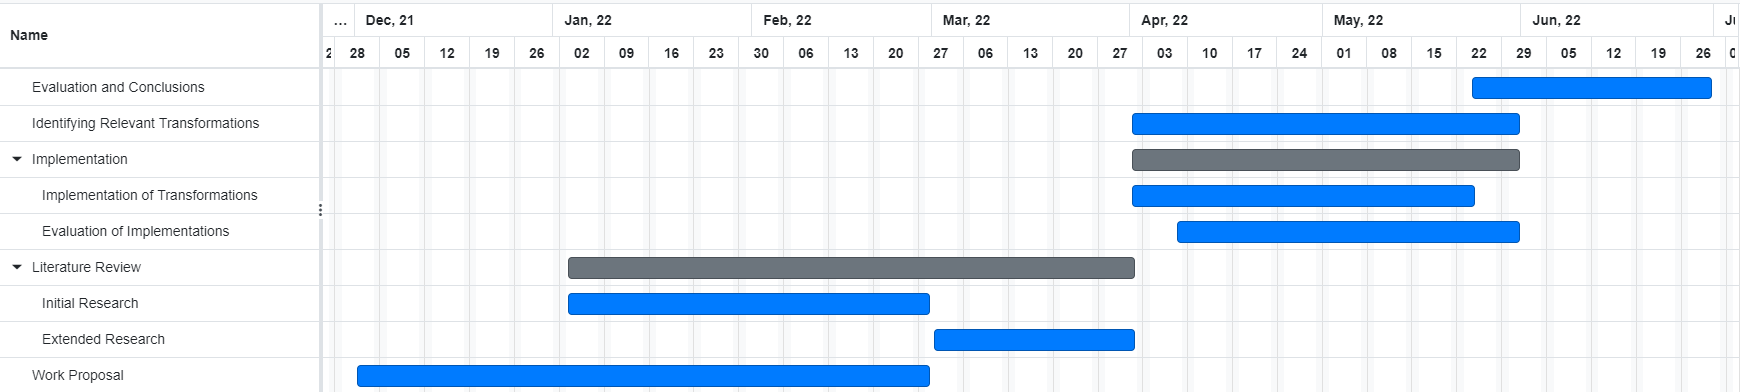
\includegraphics[width=\textwidth]{figures/gantt.png}
    \caption{Gantt chart of intended work schedule}
    \label{fig:gantt}
\end{sidewaysfigure}